\section{Frontend}
\fancyhead[RO,LE]{Frontend}

Per sviluppare il progetto abbiamo usato \anchor{\textit{Next.js}}{https://nextjs.org}, framework fullstack per lo sviluppo di applicazioni web, accompagnato da \textit{Typescript} per rendere lo sviluppo più attendibile, aggiungendo sicurezza rispetto ai tipi per tutto il codice.

Tutta la cronologia dello sviluppo è disponibile su \anchor{\textit{Github}}{https://github.com/albbus-stack/platooning-visualization} e la frontend è accessibile pubblicamente su \anchor{platooning-visualization.vercel.app}{https://platooning-visualization.vercel.app}.
Abbiamo optato per ospitare l'app su \anchor{Vercel}{https://vercel.com} dato che offre integrazione/distribuzione continua (\textit{CI}/\textit{CD}), come discuteremo in una sezione successiva.  Il rilascio della nostra applicazione non è tuttavia limitato solo a questa piattaforma ma è anche compatibile con progetti \textit{AWS Amplify} e \textit{Netlify}.

La visualizzazione della simulazione vera e propria è implementata usando \anchor{\textit{P5.js}}{https://p5js.org}, libreria che ci permette di gestire più efficientemente il rendering ad alto frame rate sul \textit{canvas HTML} e che rende disponibile una \textit{API} più ergonomica per interagire con esso.

Per gestire gli stili dell'interfaccia utente abbiamo usato \anchor{\textit{TailwindCSS}}{https://tailwindcss.com}, un framework \textit{CSS} che ci ha permesso di non dividere il codice di rendering dal codice di styling (usando il meccanismo delle classi \textit{CSS}), rendendo lo sviluppo dei componenti \textit{UI} più veloce, rintracciabile e standardizzato.

\begin{tsxCode}{Esempio di classi \textit{TailwindCSS}}
<div className="p-1 text-white transition-all duration-300 rounded-md cursor-pointer select-none bg-slate-800 hover:bg-slate-300 hover:text-slate-800">
      <InfoIcon />
</div>
\end{tsxCode}

Abbiamo reso disponibili anche varie scorciatoie da tastiera per eseguire diverse azioni nell'interfaccia utente, ad esempio \texttt{SPAZIO} mette in pausa o fa partire la simulazione. Nelle sezioni successive ne saranno definite altre in corrispondenza col loro utilizzo.

\newpage
\subsection{Impostazioni}

La gestione dello stato delle impostazioni di simulazione avviene sfruttando il \anchor{\textit{contesto React}}{https://react.dev/learn/passing-data-deeply-with-context}. Il meccanismo di funzionamento del contesto è molto simile a quello del pattern \textit{Provider}/\textit{Consumer} e si divide quindi in due parti:
\vspace{-0.2em}
\begin{itemize}
    \item \textit{Provider}: viene instanziato un componente che racchiude tutti i componenti di cui esso deve gestire lo stato, permettendo interazioni tra loro.\vspace*{-0.5em}
    \item \textit{Consumer}: per consumare (leggere) oppure aggiornare lo stato di un \textit{Provider} viene usato l'\textit{hook} \anchor{\textit{useContext}}{https://react.dev/reference/react/useContext} che espone queste funzionalità ad ogni componente sottostante al \textit{Provider}.
\end{itemize}
\vspace{-0.2em}

Nel nostro caso il \textit{DataProvider} contiene tutte le varie impostazioni della simulazione che possono essere modificate dal componente \textit{DataProvider} (la sezione che contiene i selettori orizzontali per ogni opzione ed il grafico della velocità del primo veicolo); lo stato di queste impostazioni viene in seguito letto dal \textit{canvas P5} per aggiornare la simulazione stessa. Questo meccanismo ci permette quindi di sincronizzare facilmente lo stato tra il componente di modifica e quello di visualizzazione.

Sono disponibili le seguenti impostazioni di simulazione (visibili in figura \ref{fig:simulation-settings}): \textit{Numero di veicoli}, \textit{Distanza obbiettivo tra di loro}, \textit{Distanza temporale tra di loro}, \textit{Delay di comunicazione} ed alcuni parametri del modello di platooning precedentemente discusso come \textit{Tau}, \textit{Kp} e \textit{Kd}.

\begin{figure}[H]
    \vspace{0.7em}
    \centering
    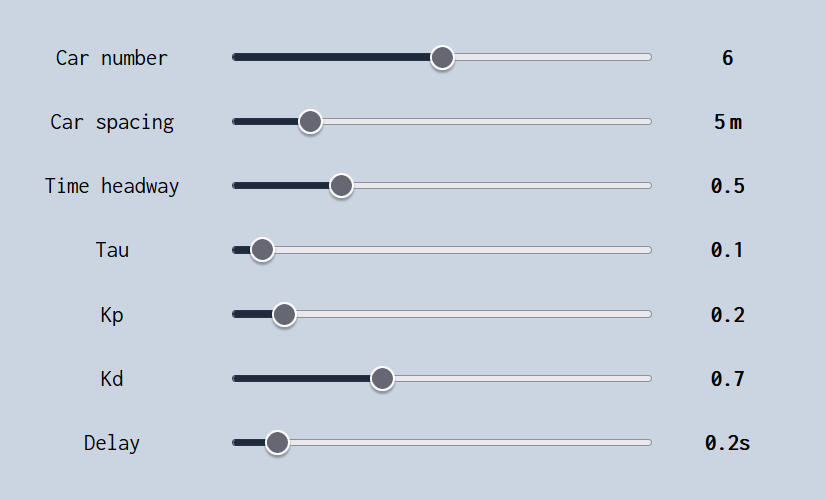
\includegraphics[width=0.75\textwidth, keepaspectratio]{images/4-frontend/simulation-settings.png}
    \caption{Varie impostazioni numeriche per la simulazione.}
    \label{fig:simulation-settings}
\end{figure}

\begin{figure}[H]
    \vspace{0.5em}
    \centering
    \captionsetup{justification=centering, margin=2cm}
    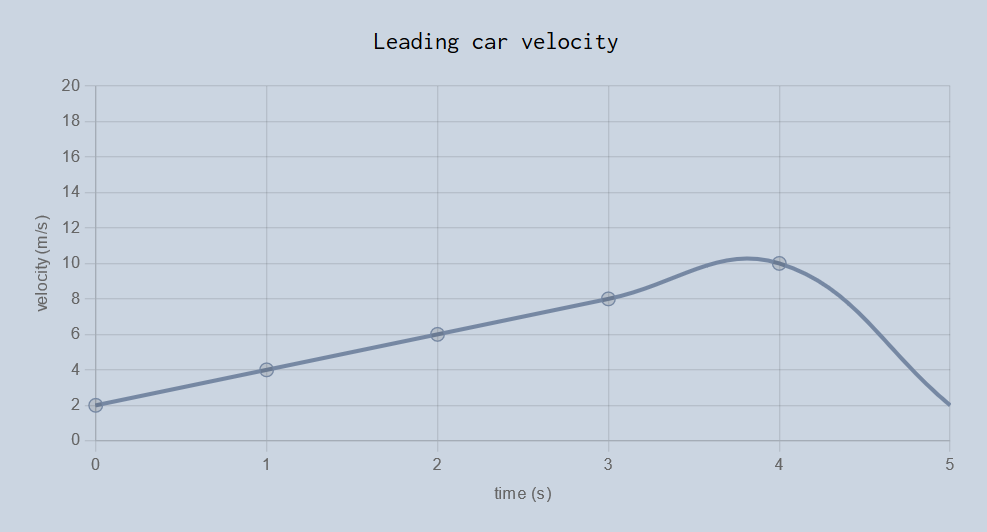
\includegraphics[width=0.75\textwidth, keepaspectratio]{images/4-frontend/velocity-settings.png}
    \caption{Grafico per impostare l'andamento del primo veicolo del convoglio nel tempo.}
    \label{fig:velocity-settings}
\end{figure}

\begin{figure}[H]
    \centering
    \captionsetup{justification=centering, margin=2cm}
    
\includegraphics[width=0.65\textwidth, keepaspectratio]{images/4-frontend/keyboard-shortcuts.png}
    \caption{Interfaccia utente per l'apertura dei pannelli (\textit{Sliver}), con sopra annotate le scorciatoie da tastiera.}
    \label{fig:keyboard-shortcuts}
\end{figure}

La velocità del primo veicolo del convoglio è controllabile tramite un grafico interattivo, in figura \ref{fig:velocity-settings}, in cui sono modificabili i punti da $t=0$ a $t=4$. Il primo veicolo segue in maniera periodica questo grafico delle velocità con accelerazione uniforme. Come descritto nella sezione successiva, è stato scelto \textit{ChartJS} per produrre anche questo grafico interattivo.

Le impostazioni per la simulazione ed i grafici risultanti sono contenute in due pannelli separati, accessibili tramite due bottoni nell'interfaccia utente (visibili in figura \ref{fig:keyboard-shortcuts}) oppure usando delle scorciatoie da tastiera: \texttt{G} per aprire il pannello dei grafici (\textit{GraphSliver}) e \texttt{S} per aprire il pannello delle impostazioni (\textit{SettingSliver}).

Dopo aver configurato i parametri desiderati, è possibile avviare la simulazione per visualizzare il comportamento del veicolo in base alle scelte effettuate. L'uso di grafici e impostazioni personalizzabili permette un'analisi interattiva del modello di platooning da parte dell'utente.

\newpage
\subsubsection*{Codice allegato}

\vspace{0.3em}
\begin{tsCode}{Gestione dello stato delle impostazioni con \textit{DataProvider}}
/* DataProvider.tsx */
export const DataProvider: React.FC<DataProviderProps> = ({ children }) => {
  const [carNumber, setCarNumber] = useState(6);
  const [carSpacing, setCarSpacing] = useState(5.0);
  const [timeHeadway, setTimeHeadway] = useState(0.5);
  const [tau, setTau] = useState(0.1);
  const [kp, setKp] = useState(0.2);
  const [kd, setKd] = useState(0.7);
  const [velocityFrameDelay, setVelocityFrameDelay] = useState(VELOCITY_DELAY);
  const [leadingCarChart, setLeadingCarChart] = useState<GraphPoints[]>(
    [0, 1, 2, 3, 4].map((i) => {
      return {
        time: i,
        velocity: i * 2 + 2,
      };
    })
  );
  ...
}

/* SettingsSliver.tsx */
const SettingsSliver: React.FC = () => {
  const { carNumber, setCarNumber, carSpacing, setCarSpacing, ... } = useContext(DataContext);
  ...
}

/* P5Canvas.tsx */
<NextReactP5Wrapper
  sketch={sketch}
  carSpacing={carSpacingSetting}
  carNumber={carNumberSetting}
  ...
>
\end{tsCode}
\vspace{0.6em}

Le varie impostazioni della simulazione sono contenute dentro \textit{DataProvider} e i loro stati sono inizializzati con dei valori di default, inclusi i punti del grafico della velocità del primo veicolo. In seguito \textit{SettingSliver} utilizza i \textit{getter} e \textit{setter} esposti da questo provider per permettere all'utente di modificare le impostazioni interattivamente attraverso gli slider.

Infine nel \textit{canvas P5} viene letto lo stato del contesto e passato all'istanza sottostante di \textit{P5.js} attraverso i \textit{props} del componente \textit{NextReactP5Wrapper} che rende la simulazione consapevole del cambiamento di qualsiasi di questi, in maniera reattiva.

\newpage
\subsection{Grafici}

La visualizzazione dei grafici è implementata usando \anchor{\textit{ChartJS}}{https://www.chartjs.org}, libreria molto popolare grazie alla performance del \textit{canvas HTML} e alla sua interazione stretta con \textit{React} (attraverso la libreria wrapper \anchor{\textit{react-chartjs-2}}{https://react-chartjs-2.js.org}).

Come suggerito precedentemente, la gestione dei dati usati per la produzione dei grafici è sempre affidata al \textit{contesto React}, in particolare al componente \textit{DataProvider} che espone \textit{getter} e \textit{setter} relativi ai dati di distanza e velocità tra i veicoli. Questo approccio ci consente di gestire in modo efficiente e organizzato tutti i dati relativi alla simulazione, garantendo una facile integrazione con il resto dell'applicazione.

La simulazione \textit{P5} stessa esegue a \textit{60 fps} e viene campionata ogni quarto di secondo ($250ms$) per raccogliere questi dati di distanza e velocità. Quando viene aggiunto un nuovo \textit{DataPoint}, i grafici contenuti in \textit{GraphSliver} si aggiornano, mostrando dinamicamente i dati raccolti, permettendo quindi agli utenti di monitorare l'evoluzione della simulazione in tempo reale. 

Nell'interfaccia utente è possibile visualizzare il grafico di distanza o velocità specifico per un veicolo; questi sono selezionabili da due dropdown presenti sopra ai grafici corrispondenti. 

E' possibile osservare un esempio della visualizzazione di questa sezione in figura \ref{fig:distance-graph} e \ref{fig:velocity-graph}.

\begin{figure}[H]
    \vspace{1em}
    \centering
    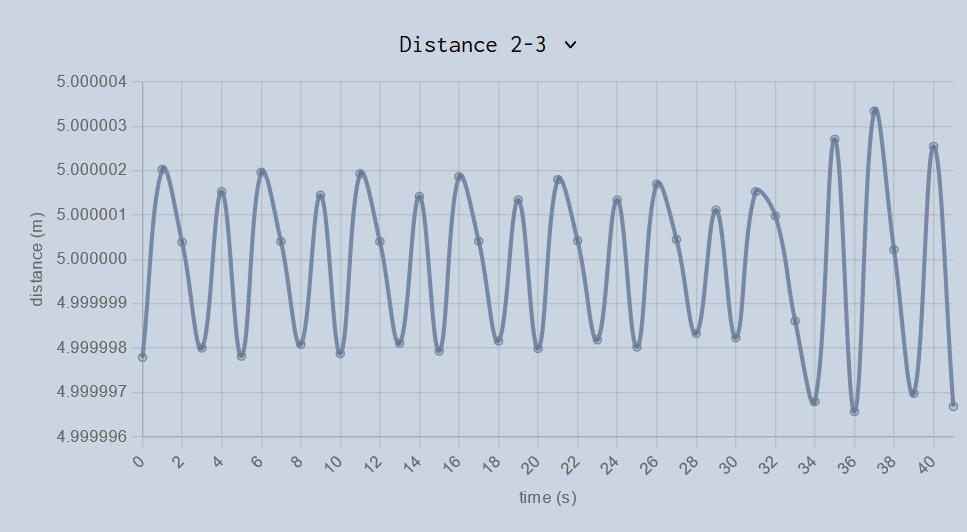
\includegraphics[width=0.85\textwidth, keepaspectratio]{images/4-frontend/distance-graph.png}
    \caption{Grafico della distanza tra due veicoli del convoglio.}
    \label{fig:distance-graph}
\end{figure}

\begin{figure}[H]
    \vspace{0.5em}
    \centering
    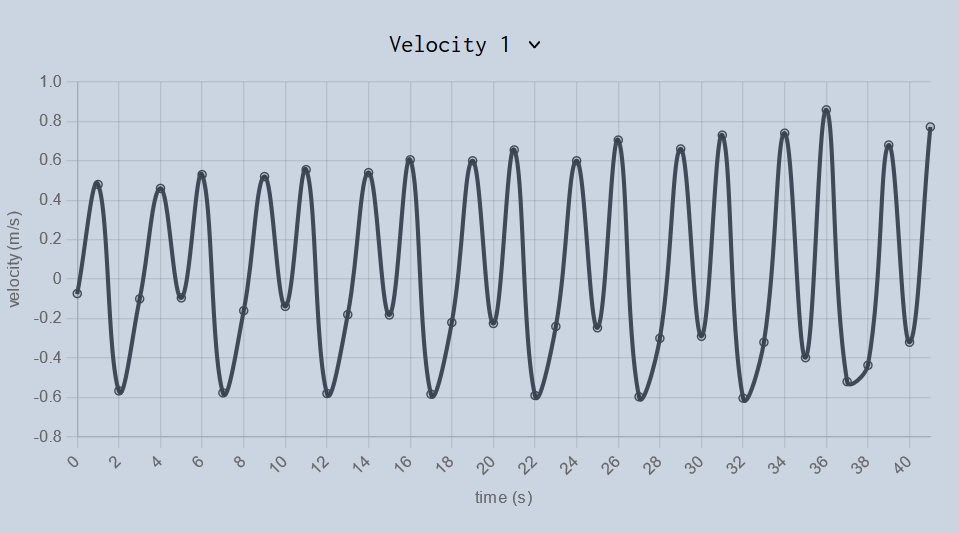
\includegraphics[width=0.85\textwidth, keepaspectratio]{images/4-frontend/velocity-graph.png}
    \caption{Grafico della velocità di un veicolo del convoglio.}
    \label{fig:velocity-graph}
\end{figure}

\begin{figure}[H]
    \centering
    \captionsetup{justification=centering, margin=3cm}
    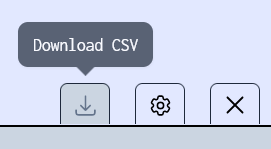
\includegraphics[width=0.55\textwidth, keepaspectratio]{images/4-frontend/csv-export.png}
    \caption{Bottone di esportazione dei dati della simulazione in \texttt{csv}.}
    \label{fig:csv-export}
\end{figure}

Un aspetto utile della nostra implementazione è la possibilità di esportare i dati raccolti in formato \texttt{csv} con la seguente struttura: \texttt{carNumber}, \texttt{time(s)}, \texttt{distance(m)}, \texttt{velocity(m/s)}. Dove \texttt{time(s)} è l'istante di tempo e \texttt{distance} si riferisce alla distanza tra il veicolo \texttt{carNumber} e \texttt{carNumber+1}. Per l'ultimo veicolo questa distanza sarà sempre considerata 0 come default dato che non c'è nessun veicolo successivo ad esso.

Il download in formato \texttt{csv} consente agli utenti di analizzare i dati della simulazione in dettaglio al di fuori dell'applicazione, utilizzando strumenti esterni o elaborando i risultati in altri contesti. In figura \ref{fig:csv-export} è visibile l'interfaccia utente per questa funzione.

\newpage
\subsubsection*{Codice allegato}

\vspace{0.3em}
\begin{tsCode}{Gestione dello stato dei grafici con \textit{DataProvider}}
/* DataProvider.tsx */
export const DataProvider: React.FC<DataProviderProps> = ({ children }) => {
  const [graphData, setGraphData] = useState([[]] as {
    distance: number;
    velocity: number;
    time: number;
  }[][]);
  ...
}

/* GraphSliver.tsx */
const GraphSliver: React.FC = () => {
  const [distanceChartIndex, setDistanceChartIndex] = useState(0);
  const [velocityChartIndex, setVelocityChartIndex] = useState(0);

  const { graphData } = useContext(DataContext);
  ...
}

/* P5Canvas.tsx */
const { setGraphData } = useContext(DataContext);

intervalRef = setInterval(() => {
  timeTick++;
  setGraphData((car) => 
    car.map((prev, i) => [ 
      ...prev, 
      { time: timeTick, distance: distance[i], velocity: velocity[i] },
    ])
  );
}, UPDATE_INTERVAL);
\end{tsCode}
\vspace{0.6em}

Come si può osservare sopra, \textit{DataProvider} contiene i dati di distanza e velocità di ogni veicolo per ogni istante di tempo. Questo stato è letto da \textit{GraphSliver} che ha due variabili di stato locali contenenti gli indici dei grafici di distanza e velocità attualmente selezionati dall'utente nella sezione corrispondente.

Lo stato del \textit{DataProvider} viene aggiornato dentro un \textit{intervallo} (cioè una \textit{API} per ripetere l'esecuzione di un blocco di codice periodicamente) nel \textit{canvas P5} che contiene i dati della simulazione in esecuzione. Nel nostro caso l'intervallo esegue ogni \texttt{UPDATE\_INTERVAL} millisecondi, costante definita precedentemente nel file ad un secondo; per ottenere dati in uscita con frequenza di campionamento più alta è sufficiente modificare questo valore.

\newpage
\subsection{Scorciatoie da tastiera}

Abbiamo aggiunto varie scorciatoie da tastiera per interagire con l'interfaccia utente più rapidamente. Segue un elenco di alcuni di questi \textit{shortcuts}: 
\begin{itemize}
\setlength{\itemsep}{-0.1em}
    \item \texttt{SPAZIO} avvia o interrompe la simulazione.
    \item \texttt{R} ripristina la simulazione alle impostazioni predefinite.
    \item \texttt{S} apre la sezione per la modifica delle impostazioni (\textit{SettingsSliver}).
    \item \texttt{G} apre la sezione di visualizzazione dei grafici (\textit{GraphSliver}).
    \item \texttt{D} scarica i dati in \texttt{csv} della simulazione eseguita.
    \item \texttt{$\uparrow$} e \texttt{$\downarrow$} ingrandiscono/diminuiscono la dimensione della \textit{Sliver}.
    \item \texttt{$\leftarrow$} e \texttt{$\rightarrow$} ciclano tra \textit{Sliver} delle impostazioni e dei grafici.
    \item \texttt{ESC} chiude la \textit{Sliver}.
\end{itemize}

\subsubsection*{Codice allegato}
\vspace{0.1em}
\begin{tsCode}{Gestione delle scorciatoie da tastiera in \textit{P5Canvas.tsx}}
useEffect(() => {  
  const onKeyDown = (e: KeyboardEvent) => {
     switch (e.key) {
      // Start/stop the simulation
      case " ":
        togglePlay();
        break;

      // Reset the simulation 
      case "r":
        resetCanvas(window.innerWidth, carNumberSetting, carSpacingSetting);
        break;
      ...
    }
  }

  document.addEventListener("keydown", onKeyDown);
  return () => document.removeEventListener("keydown", onKeyDown);
}, [togglePlay])
\end{tsCode}

% /* Sliver.tsx */
% const onKeyDown = (e: KeyboardEvent) => {
%   switch (e.key) {
%     // Download the graph data
%     case "d":
%       if (isGraphSliver && isSliverOpen) {
%         downloadGraphDataCSV(graphData);
%       }
%       break;

%     // Close the sliver
%     case "Escape":
%       setIsSliverOpen(false);
%       break;
%     ...
%   }
% }
\vspace{0.3em}

Il codice fornito gestisce le scorciatoie per \texttt{SPAZIO} e \texttt{R} utilizzando \textit{useEffect}. Con questo hook viene registrato un gestore per gli eventi \textit{keydown} quando il componente viene montato. Questo gestore di eventi controlla quale tasto è stato premuto attraverso l'oggetto \textit{KeyboardEvent} e reagisce di conseguenza. Oltre a questo \textit{useEffect} ritorna una funzione di \textit{cleanup} dove viene rilasciato il gestore delle scorciatoie.

\newpage
\subsection{Internazionalizzazione}

Per rendere questo progetto fruibile da utenti che non parlano l'inglese abbiamo deciso di implementare un sistema di internazionalizzazione che include le seguenti localizzazioni: \textit{en}, \textit{it}, \textit{fr}, \textit{es}, \textit{de}, \textit{dk}, \textit{nl}, \textit{pt}, \textit{ru}, \textit{sa}, \textit{in}, \textit{cn}, \textit{jp}, \textit{kr}.
 
Questa funzionalità è stata raggiunta usando le \anchor{\textit{Dynamic Routes}}{https://nextjs.org/docs/pages/building-your-application/routing/dynamic-routes}; queste consistono nel raccogliere il codice di rendering per varie \textit{routes} (percorsi del sito) dentro un solo componente.   
Nel nostro caso ci permettono di cambiare il linguaggio selezionato semplicemente rimandando al percorso "\texttt{/locale}" corrispondente (dove \texttt{locale} è una delle stringhe di localizzazione sopra elencate).
Per la lingua di default, cioè l'inglese, il percorso usato è "\texttt{/}" senza nessuna specificazione di lingua ulteriore, come vediamo in figura \ref{fig:dynamic-routes}.

La gestione vera e propria delle varie traduzioni è stata affidata a \anchor{\textit{ParaglideJS}}{https://inlang.com/m/gerre34r/library-inlang-paraglideJs}, un nuovo e promettente framework di internazionalizzazione. Questa libreria gestisce lo stato locale del client riguardante la lingua attualmente selezionata ed espone una semplice \textit{API} per leggerlo e modificarlo, tutto mantenendo completamente la \textit{type safety}.

Le stringhe di traduzione sono scritte in dei file \texttt{json} e possiamo aggiungere altre lingue semplicemente scrivendone uno nuovo e ricompilando il \textit{bundle} di \textit{ParaglideJS} (affinché tutte le stringhe siano controllate ed esportate staticamente prima della build del progetto).    

Per mostrare le bandiere corrispondenti ad ognuna delle lingue utilizzate abbiamo usato degli \texttt{svg} resi disponibili dalla repository \anchor{\textit{country-flags}}{https://github.com/hampusborgos/country-flags/tree/main/svg}.

\begin{figure}[H]
    \vspace{0.8em}
    \centering
    \captionsetup{justification=centering, margin=1.5cm}
    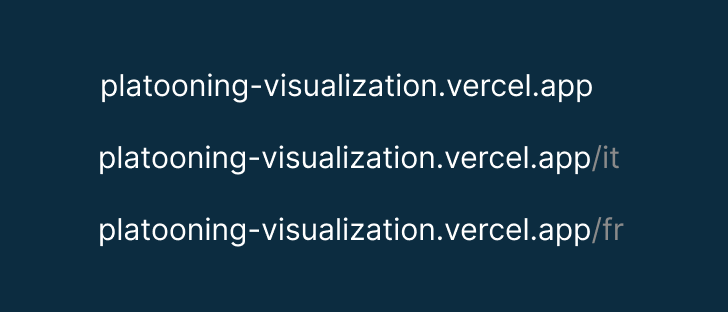
\includegraphics[width=0.7\textwidth, keepaspectratio]{images/4-frontend/dynamic-routes.png}
    \caption{Percorsi dinamici corrispondenti ad inglese (\texttt{/}), italiano (\texttt{/it}) e francese (\texttt{/fr}).}
    \label{fig:dynamic-routes}
\end{figure}

\newpage
\subsubsection*{Codice allegato}

\vspace{0.2em}
\begin{tsCode}{Utilizzo di \textit{ParaglideJS} per l'internazionalizzazione}
/* pages/[locale]/index.tsx */
import { AvailableLanguageTag, availableLanguageTags, setLanguageTag } from "../../src/paraglide/runtime";
import { useRouter } from "next/router";

const Home: NextPage = () => {
  const router = useRouter();
  const locale = router.query.locale as AvailableLanguageTag ?? "en";

  if (availableLanguageTags.includes(locale)) {
    setLanguageTag(locale);
  } else if (router.query.locale) {
    return <PageNotFound />;
  }

  return <HomePage />;
};

/* translations/it.json */
{
  "$schema": "https://inlang.com/schema/inlang-message-format",
  "title": "Simulazione di platooning",
  "graphs": "Grafici",
  "settings": "Impostazioni", ...
}

/* package.json */
{
  "name": "platooning-visualization",
  "scripts": {
    "lang": "paraglide-js compile --project ./project.inlang.json",
  }, ...
}
\end{tsCode}
\vspace{0.4em}

Come si può osservare, i percorsi dinamici sono gestiti attraverso l'\textit{hook} \anchor{\textit{useRouter}}{https://nextjs.org/docs/pages/api-reference/functions/use-router} che raccoglie la stringa corrispondente alla \textit{route} visitata nell'attributo \texttt{query.locale}. Se viene fornita una stringa vuota il \textit{type cast} la assegnerà al valore della \textit{locale} di default (\texttt{"en"}), altrimenti se viene fornita una stringa di localizzazione non valida verrà renderizzata una \textit{pagina 404} (pagina non trovata; contenente un link alla pagina principale).

Come discusso in precedenza le stringhe delle traduzioni sono contenute in dei file \texttt{json} e dobbiamo compilare i messaggi di \textit{ParaglideJS} ogni volta che queste vengono aggiornate (attraverso lo script eseguibile con \texttt{pnpm lang}).

\newpage
\subsection{Integrazione Continua}

Per garantire un flusso di sviluppo fluido e automatizzato, abbiamo configurato un sistema di integrazione continua utilizzando \textit{Vercel} e \anchor{la loro integrazione \textit{GitHub}}{https://vercel.com/docs/deployments/git/vercel-for-github}.

\textit{Vercel}, una piattaforma di hosting specializzata nel \textit{deploy} di applicazioni \textit{React} e \textit{Next.js}, offre un'integrazione continua semplice ed efficace: ogni volta che viene eseguito un commit o viene aperta una pull request sul branch principale della nostra repository viene avviato automaticamente un processo di build e distribuzione dell'applicazione.

Questo processo assicura che ogni modifica apportata al codice venga immediatamente testata e poi resa disponibile. Inoltre, \textit{Vercel} offre la funzionalità dei \textit{deployment} di preview, con la possibilità di creare anteprime delle modifiche non ancora pubblicate al pubblico, consentendo un controllo prima che queste vengano distribuite ufficialmente.

\vspace{-0.4em}
\subsubsection*{Codice allegato}

\vspace{0.3em}
\begin{tsCode}{Integrazione continua con \textit{Vercel}}
/* package.json */
{
  "name": "platooning-visualization",
  "scripts": {
    "lint": "next lint",
    "build": "pnpm lint && pnpm lang && pnpm next build",
  }, ...
}
\end{tsCode}
\vspace{0.3em}

Questo \textit{snippet} indica come vengono gestiti i passaggi di build dell'applicazione durante il processo di integrazione continua:

\vspace{-0.4em}
\begin{itemize}
\setlength{\itemsep}{-0.1em}
    \item \texttt{pnpm lint}: prima di avviare il processo di build, viene eseguito il comando di \textit{linting} per assicurarsi che il codice sia conforme agli standard definiti.
    \item \texttt{pnpm lang}: vengono poi compilate le traduzioni dell'applicazione per renderle disponibili al runtime di \textit{ParaglideJS} come discusso in precedenza.
    \item \texttt{pnpm next build}: infine viene avviato il processo di build ed esportazione dell'applicazione utilizzando \textit{Next.js}.
\end{itemize}